Consider the partial differential equation
\begin{equation}
y^2\frac{\partial^2 u}{\partial x^2}
+4y\frac{\partial^2u}{\partial x\partial y}
+\frac{\partial^2 u}{\partial y^2}=0
\label{90000001:eqn}
\end{equation}
on the domain
\[
\Omega = \{ (x,y)\,|\, y >0\}.
\]
\begin{teilaufgaben}
\item
Show that the differential equation is hyperbolic.
\item
Find the differential equation for the characteristics.
\item
The differential equation for the characteristics is an ordinary
differential equation of first order for two unknown functions
$x(s)$ and $y(s)$.
Factorize the equation into two factors of the form
\[
(\dot x(s)-ry(s)\dot y(s))\cdot (\dot x(s)-qy(s)\dot y(s)),
\]
then determine $r$ and $q$.
\item
Find the equation for the characteristics by solving the ordinary
differential equations
\begin{align*}
\dot x(s) - ry(s)\dot y(s)&=0\qquad\text{und}\\
\dot x(s) - qy(s)\dot y(s)&=0,
\end{align*}
use 
$\frac{d}{ds}(y(s)^2)=2y(s)\dot y(s)$
in the process.
\end{teilaufgaben}

\begin{loesung}
\begin{teilaufgaben}
\item
The determinant of the symbol matrix $A$ is
\[
A=\begin{pmatrix}
y^2&2y\\
2y&1
\end{pmatrix}
\quad\Rightarrow\quad
\det (A)=y^2-4y^2=-3y^2<0 \quad\text{in $\Omega$},
\]
thus the equation is hyperbolic.
\item
From the coefficients of the symbol matrix, we can find the equation
\[
y(s)^2\dot y(s)^2-4y(s)\dot x(s)\dot y(s)+\dot x(s)^2=0
\]
for the characteristics.
\item
Factorizing as proposed in the problem gives
\begin{align*}
0&=(\dot x(s)-ry(s)\dot y(s))(\dot x(s)-qy(s)\dot y(s))
\\
&=\dot x(s)^2-(r+q)\dot x(s) y(s)\dot y(s)+rqy(s)^2\dot y(s)^2.
\end{align*}
The numbers $r$ and $q$ must satisfy the equation
\begin{align*}
r+q&=4\\
rq&=1.
\end{align*}
By substituting
$q=1/r$ in the first equation, we get
\begin{align*}
r+\frac1r&=4\\
r^2-4r+1&=0.
\end{align*}
This quadratic equation has the solutions
\begin{equation}
r
=
2\pm\sqrt{4-1}
=
\begin{cases}
\phantom{-}\sqrt{3}+2\phantom{.}\\
         - \sqrt{3}+2.
\end{cases}
\label{90000001:r}
\end{equation}
\item
The ordinary differential equation is
\[
\dot x(s)=ry(s)\dot y(s)=\frac{r}{2}\frac{d}{ds}(y(s)^2).
\]
Integrating with respect to $s$ gives
\[
x(s) + C=\frac{r}{2}y(s)^2.
\]
Because of $y(s)>0$, the only possibility for $y$ is
\[
y = \sqrt{\frac{2}{r}(x+C)}.
\]
The characteristics thus satisfy an equation of the form
\begin{equation}
\frac{r}2y^2-x-C=0,
\label{90000001:parabola}
\end{equation}
these are parabolas.
\end{teilaufgaben}
\begin{figure}
\centering
\definecolor{darkgreen}{rgb}{0,0.6,0}
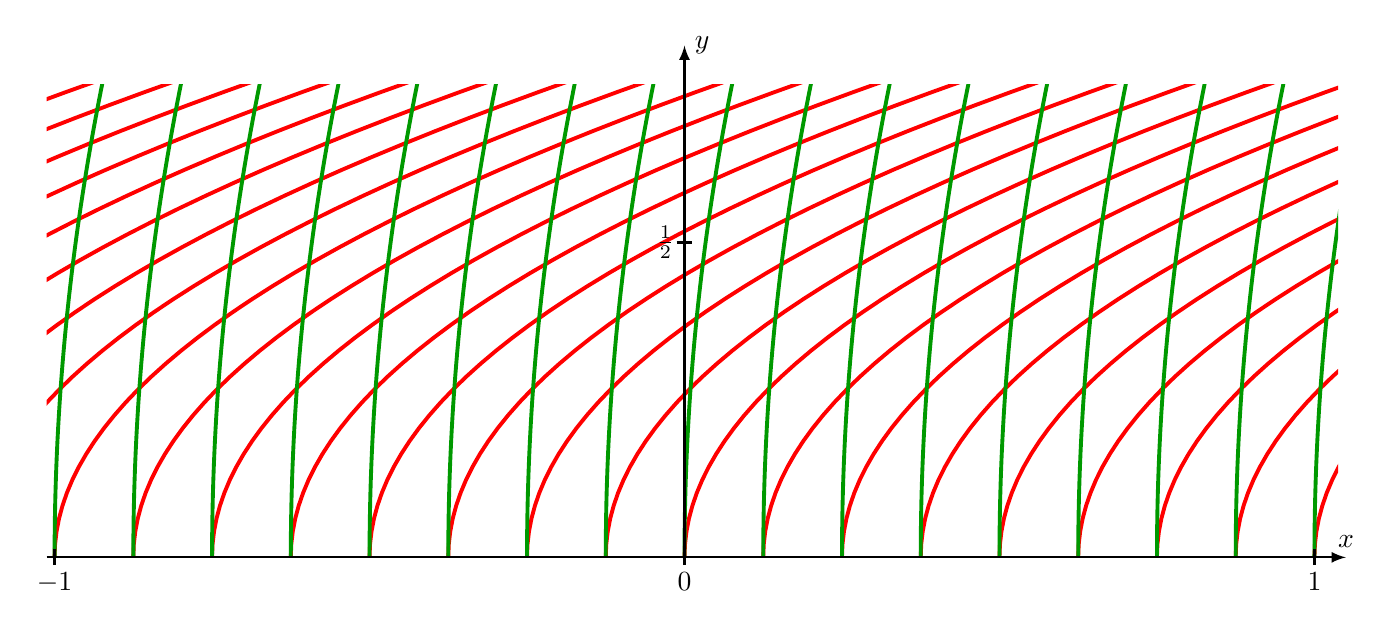
\begin{tikzpicture}[>=latex,thick]
\pgfmathparse{sqrt(3)+2}
\xdef\rplus{\pgfmathresult}
\pgfmathparse{-sqrt(3)+2}
\xdef\rminus{\pgfmathresult}
\begin{scope}
\clip (-8.1,0) rectangle (8.3,6);
\foreach \s in {-16,...,8}{
	\draw[color=red,line width=1.4pt] plot[domain=0:0.8,samples=40]
		({\s+8*0.5*\rplus*\x*\x},{8*\x});
}
\foreach \s in {-16,...,8}{
	\draw[color=darkgreen,line width=1.4pt] plot[domain=0:0.8,samples=40]
		({\s+8*0.5*(1/\rplus)*\x*\x},{8*\x});
}
\end{scope}
\draw[->] (-8.1,0) -- (8.4,0) coordinate[label={$x$}];
\draw[->] (0,-0.1) -- (0,6.5) coordinate[label={right:$y$}];
\draw (8,-0.1) -- (8,0.1);
\draw (-8,-0.1) -- (-8,0.1);
\node at (8,0) [below] {$1$\strut};
\node at (0,0) [below] {$0$\strut};
\node at (-8,0) [below] {$-1$\strut};
\draw (-0.1,4) -- (0.1,4);
\node at (0,4) [left] {$\frac12$};
\end{tikzpicture}
\caption{Characteristics of the differential equation~\eqref{90000001:eqn}
are parabolas given by \eqref{90000001:parabola} for the two values
of $r$ found in \eqref{90000001:r}, red parabolas for $r=\sqrt{3}+2$ and
green parabolas for $r=-\sqrt{3}+2$.
\label{90000001:char}}
\end{figure}
The problem does not ask to compute the characteristics through a given
point $(x_0,y_0)$, we nevertheless present a solution for this here.
For the characteristics for the factors $r$ and $q$ the constants
$C_r$ and $C_q$ are
\[
C_r=\frac{r}{2}y_0^2-x_0
\qquad
\text{and}
\qquad
C_q=\frac{q}{2}y_0^2-x_0
\]
respectively.
This means that the characteristics through 
$(x_0,y_0)$ are
\begin{align*}
y&=\sqrt{
\frac2r(x+C_r)
}
=
\sqrt{
\frac2r(x+
\frac{r}{2}y_0^2-x
)
}
=\sqrt{y_0^2+\frac2r(x-x_0)}
\qquad\text{and}
\\
y&
=\sqrt{y_0^2+\frac2q(x-x_0)}
\end{align*}
respectively.
\end{loesung}
